\documentclass[11pt]{article}

% --- packages -------------------------------------------------------------------------------
\usepackage[margin=1in]{geometry}
\usepackage{amsmath,amssymb,bm}
\usepackage{graphicx}
\usepackage{booktabs}
\usepackage{threeparttable}
\usepackage{subcaption}
\usepackage[font=small,labelfont=bf]{caption}
\usepackage{enumitem}
\usepackage{xcolor}
\usepackage[colorlinks=true,allcolors=blue!55!black]{hyperref}

\graphicspath{{figures/}}

% --- notation (mirrors the JGCD baseline) ---------------------------------------------------
\newcommand{\norm}[1]{\left\lVert#1\right\rVert}
\newcommand{\Real}{\mathbb{R}}
\newcommand{\xcl}{\bm{x}_{cl}}
\DeclareMathOperator{\tr}{tr}
\DeclareMathOperator{\rank}{rank}
\DeclareMathOperator*{\minimize}{minimize}
\newcommand{\st}{\ \text{subject to}\ }
\newcommand{\Wstlog}{\bm{W}^{(r)}_{\bm{\Sigma}^{-1}}}
\newcommand{\Lf}{L_{\bm{f}}}
\newcommand{\code}[1]{\texttt{\small #1}}

\title{\textbf{Improving the Beginner's Observability-Aware Control}\\[2pt]
  \large Real-time solve and constraint-lean reformulation for range-only cooperative
  navigation}
\author{H.\ S.\ Helson Go}
\date{\today}

\begin{document}
\maketitle

\begin{abstract}
\noindent The baseline observability-aware control (OAC) of Ref.~\cite{jgcd} maximizes the
short-time local observability Gramian (STLOG) of a range-only quadrotor cooperative-localization
system, and is validated as an \emph{offline} guidance planner: its nonlinear program (NLP) takes
seconds to solve. This report takes that baseline as a starting point and reports two unambiguous
advances toward online execution. First, a smooth Gramian surrogate restores a usable gradient
where the baseline's per-node minimum-eigenvalue objective is numerically degenerate, and pairing
it with an early-stopped sequential-quadratic-programming (SQP) solver brings the per-tick solve
from seconds to $\sim\!100$\,ms while holding full observability---an $\sim\!20$--$90\times$
speedup over the published solve time. Second, folding the hard inter-vehicle distance constraint
into the objective as a one-sided penalty reduces the active-set NLP to a box-bounded
unconstrained solve that is faster, feasible, and fully just-in-time compilable. Both advances are
produced programmatically by sweeping two headline examples with Hydra; we report ablation tables,
world-frame trajectories, and metric time-series. We then isolate, but do not yet resolve, the
central robustness gap---\emph{carried} estimation in the loop: a controller acting on its own
drifting estimate destabilizes the estimator it relies on. A three-way diagnostic localizes the
cause (carried estimator mean plus loop-closing, neither of which the paper's re-anchored
validation exercises), and we lay out a research plan to address it.
\end{abstract}

% ============================================================================================
\section{Introduction}\label{sec:intro}

A cooperative localization system (CLS) lets a follower drone recover its position relative to a
leader from inter-vehicle range alone, a low-cost surrogate for GNSS in denied
environments~\cite{jgcd}. A one-dimensional range does not, by itself, fix the follower's relative
position; the follower must \emph{move} to render its state observable. The baseline OAC of
Ref.~\cite{jgcd} formalizes this as an optimal predictive control (OPC) problem that maximizes the
STLOG of the range-only CLS, and demonstrates that the resulting orbiting motion sharply improves
estimation precision over a rigid straight-line formation. That baseline is deliberately
conservative: it runs the OPC offline.

Reproducing it on the identical relative-pose model surfaces several obstacles to real-time,
closed-loop use. This report reports two that are now \emph{unambiguously} addressed, and isolates
a third that is not:
\begin{itemize}[leftmargin=1.6em,itemsep=2pt]
  \item \textbf{Slow solve, long ticks (Sec.~\ref{sub:p1}, \ref{sub:res-solve}).} The order-$5$,
    $N=20$ NLP solves in seconds. A smooth surrogate objective and an early-stopped SQP bring it
    to $\sim\!100$\,ms at full observability.
  \item \textbf{Hard nonlinear constraints force an NLP (Sec.~\ref{sub:p4},
    \ref{sub:res-solve}).} The inter-vehicle distance band is a hard nonlinear constraint; a
    one-sided penalty reduces the problem to a box-bounded unconstrained solve.
  \item \textbf{Carried estimation in the loop (Sec.~\ref{sec:future}).} Closing the control loop
    on a carried EKF estimate destabilizes the estimator---the open problem, which the paper's
    re-anchored validation never exercises.
\end{itemize}
The study is reproducible: a single Hydra sweep (\code{report/sweep.sh}) over two headline
examples emits every number and figure herein.

% ============================================================================================
\section{The Baseline OAC}\label{sec:baseline}

We retain the baseline's model and notation verbatim~\cite{jgcd}. The relative state of the
follower with respect to the leader is $\bm{x} = [\bm{r}^\top\ \bm{q}^\top\ \bm{v}^\top]^\top
\in \Real^{10}$, stacking the body-frame relative position $\bm{r}$, the relative attitude
quaternion $\bm{q}\in\mathcal{S}^3$, and the body-frame relative velocity $\bm{v}$; the input
$\bm{u} = [\bm{u}_l^\top\ \bm{u}_f^\top]^\top \in \Real^{8}$ stacks the leader and follower
thrust/body-rate commands $\bm{u}_i = [f_i\ \bm{\omega}_i^\top]^\top$. The relative motion model is
\begin{equation}\label{eq:dyn}
  \dot{\bm{x}} = \bm{f}(\bm{x},\bm{u}) \triangleq
  \begin{bmatrix}
    \bm{r}^\times\bm{\omega}_l + \bm{v} \\[2pt]
    -\tfrac{1}{2}\mathcal{I}^\star(\bm{\omega}_f)\otimes\bm{q}
      + \tfrac{1}{2}\bm{q}\otimes\mathcal{I}^\star(\bm{\omega}_l) \\[2pt]
    \bm{v}^\times\bm{\omega}_f + k_l f_l\,\bm{R}(\bm{q})\bm{1}_3 - k_f f_f\,\bm{1}_3
  \end{bmatrix},
\end{equation}
with $\bm{R}(\cdot)$ the quaternion rotation matrix, $\otimes$ the Hamilton product,
$\mathcal{I}^\star(\cdot)$ the pure-imaginary embedding, and $(\cdot)^\times$ the cross-product
matrix. The measurement is range-and-attitude,
\begin{equation}\label{eq:obs}
  \bm{y} = \bm{h}(\bm{x}) \triangleq
  \begin{bmatrix} \tfrac{1}{2}d^2 \\ \bm{q} \end{bmatrix} \in \Real^{5},
  \qquad d = \norm{\bm{r}},
\end{equation}
whose Jacobian $\partial\bm{h}/\partial\bm{x}$ is zero in the velocity block: the relative
velocity is observable only \emph{indirectly}, through the motion, which is exactly what makes the
problem interesting.

\paragraph{Observability measure.} Observability is quantified by the order-$r$ STLOG, built from
Lie derivatives of $\bm{h}$ along $\bm{f}$ over a short horizon $T$:
\begin{equation}\label{eq:stlog}
  \Wstlog(\bm{x},\bm{u};T) =
  \sum_{i,j=0}^{r} \frac{T^{\,i+j+1}}{(i+j+1)\,i!\,j!}\,
  D\!\left(\Lf^i\bm{h}\right)^{\!\top}\bm{\Sigma}^{-1} D\!\left(\Lf^j\bm{h}\right),
\end{equation}
with $\bm{\Sigma}$ the measurement covariance. When the order meets the local observability index,
$r \ge r_*(\bm{x},\bm{u})$, the smallest eigenvalue is positive but scales as
$\lambda_{\min}(\Wstlog) = C(\bm{x},\bm{u};T)\,T^{\,2r_*+1}$; for the range-only quadrotor CLS
$r_* \ge 5$, so the floor is $T^{11}$. The baseline objective maximizes the per-node worst observable
direction (E-optimality), summed over the horizon:
\begin{equation}\label{eq:Vbase}
  V(\bm{x},\bm{u}) = \sum_{k=0}^{N-1}
  \lambda_{\min}\!\big(\Wstlog(\bm{x}^*(T_k),\bm{u}(T_k))\big).
\end{equation}

\paragraph{OPC problem.} The receding-horizon controller solves, at the current state $\xcl$,
\begin{equation}\label{eq:opc}
  \minimize_{\bm{u}_{0:N-1}}\ \frac{1}{V(\bm{x},\bm{u}) + c}
  \quad\st
  \begin{cases}
    \bm{x}_{k+1} = \bm{f}_{\mathrm d}(\bm{x}_k,\bm{u}_k),\ \ \bm{x}_0 = \xcl,\\
    u_{\min,i} \le u_{k,i} \le u_{\max,i},\\
    d_{\min} \le d_k \le d_{\max},
  \end{cases}
\end{equation}
with $c=10^{-6}$ and the inter-vehicle distance band $[d_{\min},d_{\max}]$. The baseline solves
\eqref{eq:opc} with a trust-region SQP at $r=5$, $N=20$, $T=0.2$\,s, integrator step $0.05$\,s---reported
at $2$--$4$\,s per solve (Table~1 of Ref.~\cite{jgcd}), i.e.\ an offline guidance
planner.\footnote{Our re-measurement of the unmodified solver on the same model is $\sim\!10$\,s
per solve; the published $2$--$4$\,s reflects looser tolerances. Either way the gap to a $10$\,Hz
tick is 2--3 orders of magnitude.} Crucially, the paper validates the estimator by propagating the
EKF \emph{covariance} along this fixed offline trajectory with the mean re-anchored to truth---it
never closes the control loop on a carried estimate (Sec.~\ref{sec:future}).

% ============================================================================================
\section{Two Obstacles, Addressed}\label{sec:problems}

\subsection{Slow solve, long ticks}\label{sub:p1}
Profiling the baseline solve attributes $\sim\!94\%$ of wall time to the SQP solver's own
internals and only $\sim\!6\%$ to evaluating the STLOG and its gradient: accelerating the Gramian
is a dead end. There is also a \emph{numerical} defect in the objective. By the $T^{11}$ floor of
\eqref{eq:Vbase}, at the operating point $\lambda_{\min}(\Wstlog)\sim10^{-13}$ with a gradient of
the same order---the objective is flat and the solver stalls. The lever is the \emph{objective and
the solver}, not the observability kernel.

\subsection{Hard nonlinear constraints force an NLP}\label{sub:p4}
The distance band $d_{\min}\le d_k\le d_{\max}$ is a nonconvex nonlinear constraint, forcing an
active-set NLP with constraint Jacobians evaluated every iteration. When the objective rides the
constraint boundary (as D-optimality does), each iteration pays for an active inequality. A solver
without active-set machinery---hence fully just-in-time (JIT) compilable, a step toward a
hardware-deployable kernel---is preferable if feasibility can be preserved.

% ============================================================================================
\section{Methods}\label{sec:methods}

\paragraph{Smooth surrogates.} We replace the degenerate per-node $\lambda_{\min}$ with smooth
spectral surrogates of the per-node Gramian---the log-determinant (D-optimality) and the
soft-minimum eigenvalue (smooth E-optimality):
\begin{equation}\label{eq:surrogates}
  J_{\log} = -\sum_{k}\sum_{i} \log(\lambda_i + \epsilon),
  \qquad
  J_{\mathrm{sm}} = \sum_{k} \tau\log\sum_{i} e^{-\lambda_i/\tau},
\end{equation}
with $\lambda_i$ the eigenvalues of $\Wstlog$ at node $k$. Minimizing $J_{\mathrm{sm}}$ recovers
$\lambda_{\min}$-maximization as $\tau\!\to\!0$ but with a usable gradient at degeneracy; both
restore an $O(1)$ gradient ($\norm{\nabla J_{\log}}\approx 7.8$) where the baseline measures
$\sim\!10^{-13}$, and drive the trajectory from $4$ to the full $6$ observable directions.

\paragraph{Lean, early-stopped solver.} We solve \eqref{eq:opc} with SQP capped at six iterations
and warm-started by shift-appending the previous solution. The objective and its gradient are
JIT-compiled once and runtime arguments are threaded as traced inputs, so no per-tick
recompilation occurs. Early stopping is not a sacrifice: observability plateaus within $\sim\!6$
iterations, so the cap is ``free.''

\paragraph{Soft constraint.} The distance band is folded into the objective as a smooth one-sided
penalty,
\begin{equation}\label{eq:penalty}
  J_{\mathrm{pen}}(\bm{u}) = w_p \sum_k \Big[\max(c_k - d_{\max}^2,\,0)^2
  + \max(d_{\min}^2 - c_k,\,0)^2\Big], \quad c_k = d_k^2,
\end{equation}
and the problem is then solved as a box-bounded unconstrained minimization (L-BFGS-B), removing the
active-set QP entirely.

% ============================================================================================
\section{Results}\label{sec:results}

All numbers and figures are produced by \code{report/sweep.sh}, which sweeps the two headline
examples with Hydra and dumps per-run records; \code{report/tabulate.py} and
\code{report/figures.py} render the tables and plots. The quadrotor runs at $r=5$, $N=20$,
$T=0.2$\,s, step $0.05$\,s on CPU; the planar leader-follower at order $1$, $N=5$.

\subsection{Real-time solve and the soft constraint}\label{sub:res-solve}
Table~\ref{tab:solve} reports the quadrotor open-loop orbit (Fig.~\ref{fig:quad-orbit}). The smooth
soft-min objective with SQP-at-6 brings the median per-tick solve to $\sim\!0.12$\,s---inside an
order of magnitude of the $10$\,Hz target and $\sim\!20$--$30\times$ faster than the published
baseline (Sec.~\ref{sec:baseline})---while holding full $6/6$ observability and the distance band.
The soft penalty \eqref{eq:penalty} cuts the median solve by a further third (no active-set QP)
with no band violation. The planar case (Table~\ref{tab:planar}) clears $10$\,Hz outright at
$\sim\!3$\,ms; there the observability-aware follower drives the unobservable initial error down
$\sim\!3.3\times$ in RMSE and $\sim\!5\times$ in final error where a straight-flying follower
cannot (Figs.~\ref{fig:planar-spatial}--\ref{fig:planar-ts}), and the soft constraint composes
with both the log-det and the balanced objective.

\begin{table}[t]
  \centering
  \caption{Per-tick solve and observability, quadrotor open-loop orbit. Compile is the one-time
    tick-$0$ JIT cost; $d$ range is the realized inter-vehicle distance against the $[1,2]$\,m
    band. The soft penalty is faster with no band violation.}
  \label{tab:solve}
  \begin{threeparttable}
    \footnotesize\setlength{\tabcolsep}{4.5pt}
    \begin{tabular}{llllrrrcc}
\toprule
Case & Objective & Solver & Constr. & Median & p95 & Compile & Obs.\ dirs & $d$ range \\
 & & & & [ms] & [ms] & [s] & & [m] \\
\midrule
JGCD baseline OPC\textsuperscript{a} & min-eig & trust-constr & hard & $2000$--$4000$ & --- & --- & $6/6$ & $[1,3]$ \\
Open-loop orbit & soft-min & SLSQP@6 & hard & 124 & 207 & 27.0 & $6/6$ & $[1.35,\,2.01]$ \\
Open-loop orbit & soft-min & SLSQP@6 & soft & 84 & 144 & 26.4 & $6/6$ & $[1.31,\,2.01]$ \\
\bottomrule
\end{tabular}
    \begin{tablenotes}\footnotesize
      \item[a] Identical OPC solved offline; solve time from Table~1 of Ref.~\cite{jgcd}.
    \end{tablenotes}
  \end{threeparttable}
\end{table}

\begin{figure}[t]
  \centering
  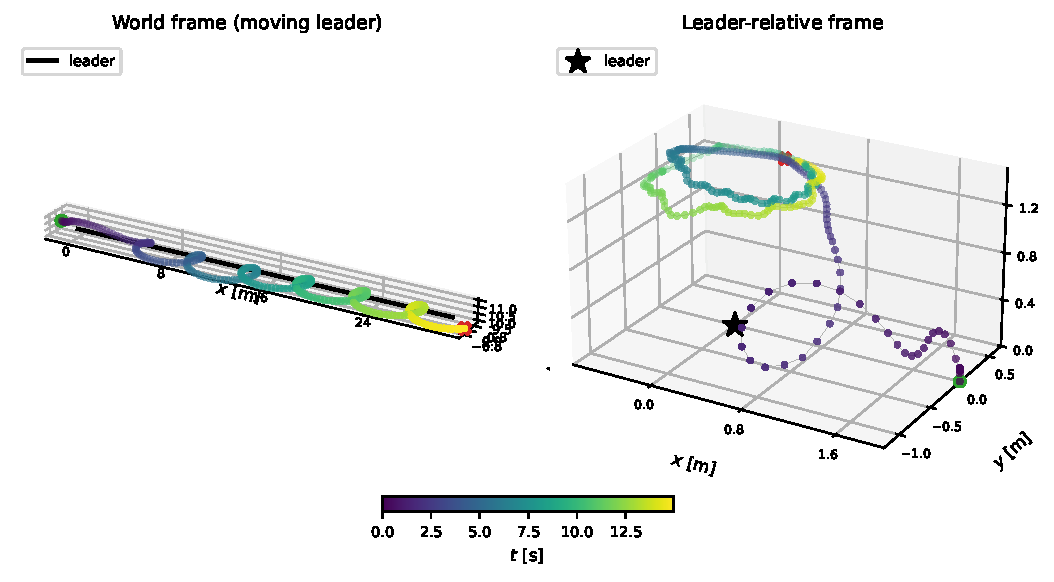
\includegraphics[width=\textwidth]{quad_orbit.pdf}
  \caption{Quadrotor open-loop observability orbit (soft-min + SQP-at-6, perfect feedback,
    level-cruising leader). \emph{Left}: world-frame trajectory---the follower orbits the leader
    into a constant-radius helix. \emph{Right}: the same motion in the leader-relative frame.}
  \label{fig:quad-orbit}
\end{figure}

\begin{table}[t]
  \centering
  \caption{Planar leader-follower, carried EKF, $120$ steps. Follower-position RMSE and final
    error vs.\ a no-OAC (straight-flying) follower; the no-OAC baseline is scheme-independent.
    $\lambda_{\min}$ is the median accumulated-Gramian margin. The planar unicycle is robustly
    observable, unlike the quadrotor (Sec.~\ref{sec:future}).}
  \label{tab:planar}
  \begin{tabular}{lrrrr}
\toprule
Configuration & RMSE & Final $\|e\|$ & Median solve & $\lambda_{\min}$ \\
 & [m] & [m] & [ms] & \\
\midrule
No-OAC (drive straight) & 0.80 & 0.79 & --- & --- \\
\midrule
OAC log-det & 0.24 & 0.16 & 2.7 & 3.27 \\
OAC log-det, soft & 0.63 & 0.25 & 2.3 & 2.27 \\
OAC balanced & 0.45 & 0.16 & 0.8 & 0.11 \\
OAC balanced, soft & 0.51 & 0.17 & 1.5 & 0.16 \\
\bottomrule
\end{tabular}
\end{table}

\begin{figure}[t]
  \centering
  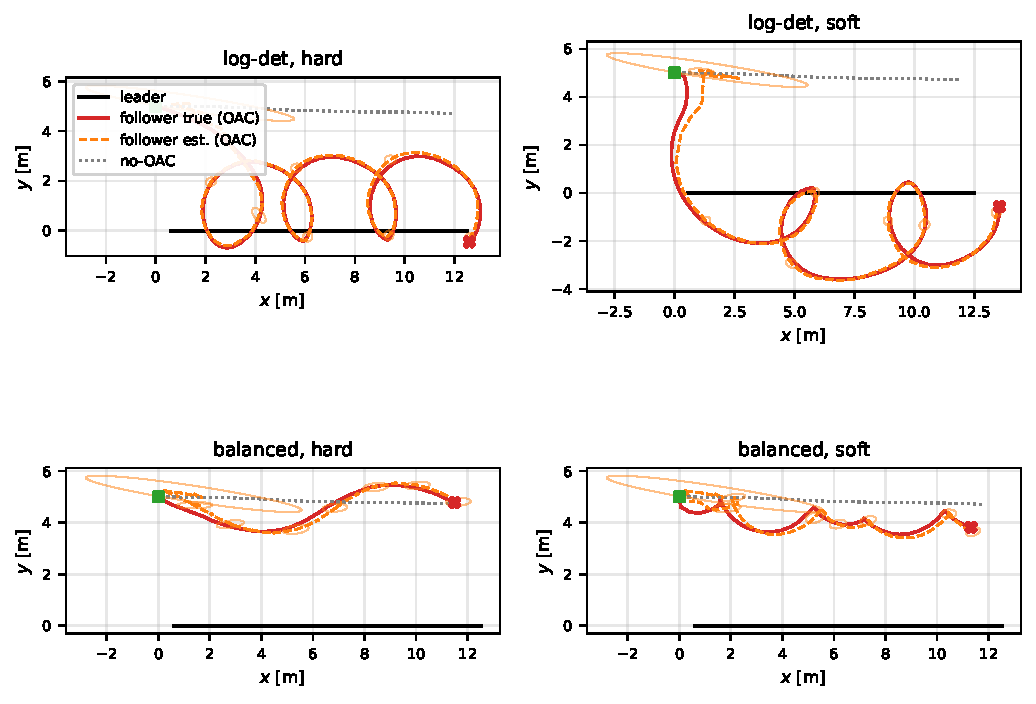
\includegraphics[width=\textwidth]{planar_spatial.pdf}
  \caption{Planar world-frame trajectories with $3\sigma$ covariance ellipses. Log-det induces
    aggressive observability orbits; the balanced cost yields gentle formation-keeping with mild
    excitation. The no-OAC follower (dotted) drives straight and never localizes. The soft
    constraint composes with both objectives.}
  \label{fig:planar-spatial}
\end{figure}

\begin{figure}[t]
  \centering
  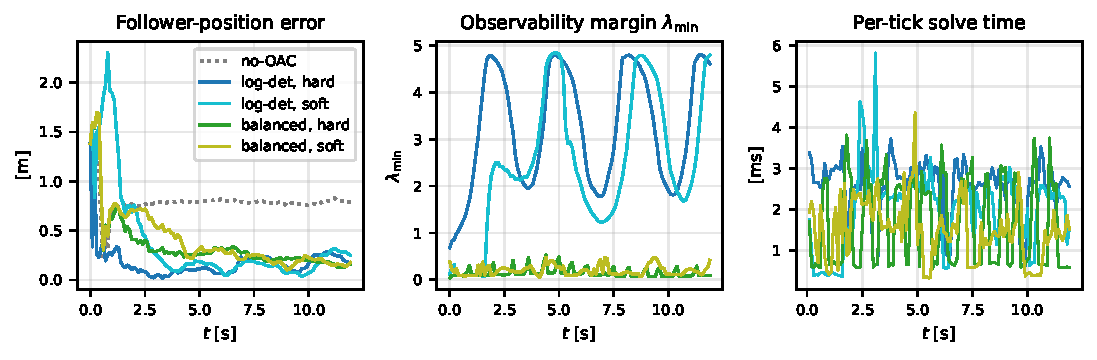
\includegraphics[width=\textwidth]{planar_timeseries.pdf}
  \caption{Planar metrics across configurations. Every OAC variant drives the initial error down
    where no-OAC (dotted) cannot; the observability margin shows log-det spending heavily on
    excitation while the balanced schemes stay low; all solve in a few milliseconds.}
  \label{fig:planar-ts}
\end{figure}

% ============================================================================================
\section{Open Problem and Plan: Carried Estimation in the Loop}\label{sec:future}

The advances above concern the \emph{planner}. The central robustness gap is the \emph{estimator}:
what happens when the controller acts on a carried estimate rather than truth. The paper sidesteps
this---its quadrotor estimator validation propagates the EKF covariance along the fixed offline
trajectory with the \emph{mean re-anchored to the true state each step}, so the mean never drifts
and divergence is impossible by construction. A real receding-horizon controller has no truth to
re-anchor to.

A three-way diagnostic on the same pure-observability OA trajectory (moving leader, $80$ steps,
five seeds) isolates the cause (Table~\ref{tab:trichotomy}, Fig.~\ref{fig:trichotomy}). Re-anchoring
the mean to truth (the paper's setup) stays robustly bounded across seeds---error $\sim\!0.4$\,m,
NEES at or below its $\chi^2_9$ band (conservative)---confirming the trajectory \emph{is}
observable. Merely \emph{carrying} the mean while still planning on truth breaks consistency: the
NEES rises into the dozens, though the error stays bounded over five seeds. \emph{Closing} the
loop---planning on the carried estimate---is catastrophic in the worst case: a seed's
relative-position error escapes past several metres and its normalized estimation-error-squared
(NEES) exceeds $900$, two orders of magnitude beyond the band. The covariance the controller trusts
shrinks faster than the true error grows---a confident-wrong divergence that covariance-based
scheduling cannot detect, since it keys on claimed uncertainty rather than estimator surprise. The
planar unicycle (Table~\ref{tab:planar}) does \emph{not} exhibit this: its lower-dimensional,
range-only geometry is robustly observable, so its carried closed loop is stable. The quadrotor's
coupling is the open problem.

\begin{table}[h]
  \centering
  \caption{Carried-estimation trichotomy, quadrotor pure-observability trajectory ($5$ seeds,
    moving leader). NEES median/worst over seeds against the $\chi^2_9$ band $[2.7,19]$ (below the
    band is conservative, far above is divergent); ``Div.'' flags any seed whose error exceeds
    $5$\,m. Carrying the mean and closing the loop are what destabilize.}
  \label{tab:trichotomy}
  {\small\setlength{\tabcolsep}{4.5pt}\begin{tabular}{lllrrrc}
\toprule
Setup & EKF mean & Plans on & NEES & NEES & $\|e\|_{\max}$ & Div. \\
 & & & med. & worst & med.\ [m] & \\
\midrule
Re-anchor mean to truth (paper) & truth (pinned) & $\approx$truth & 2 & 2 & 0.36 & -- \\
Carry mean, plan on truth & carried & truth & 44 & 112 & 1.59 & -- \\
Carry mean, plan on estimate & carried & estimate & 44 & 941 & 1.58 & \checkmark \\
\bottomrule
\end{tabular}
% chi^2_9 band [2.7, 19.0]; NEES<band = conservative, >>band = divergent}
\end{table}

\begin{figure}[h]
  \centering
  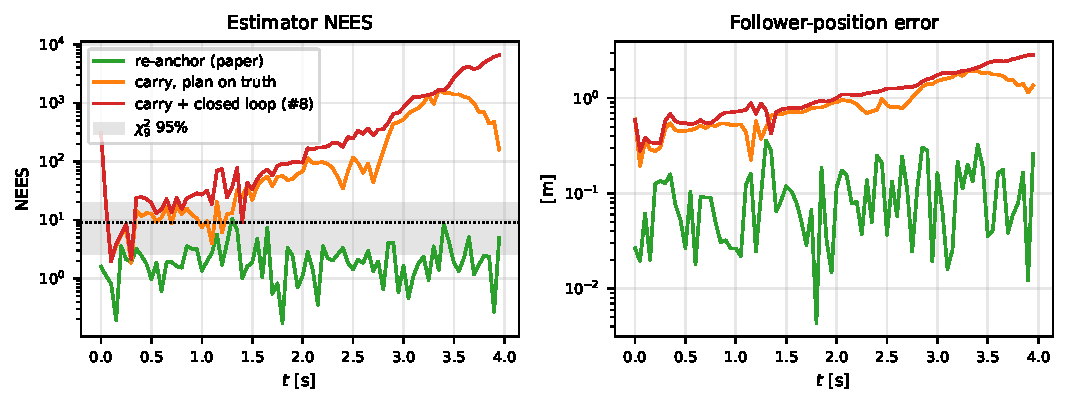
\includegraphics[width=\textwidth]{quad_trichotomy.pdf}
  \caption{Estimator NEES (left) and follower-position error (right) for the three setups (seed
    $0$). Re-anchoring stays in the $\chi^2_9$ band (shaded); carrying the mean drifts; closing the
    loop diverges.}
  \label{fig:trichotomy}
\end{figure}

\paragraph{Plan.} The detailed research plan lives in \code{docs/carried\_estimation\_plan.md}; in
brief, ranked by expected leverage:
\begin{enumerate}[leftmargin=1.8em,itemsep=1pt]
  \item \textbf{Estimator consistency first.} The divergence is confident-wrong, so the EKF is
    overconfident in the weakly observable directions. Evaluate an observability-constrained /
    consistency-preserving EKF and process-noise inflation before any control change; a consistent
    filter is a precondition for trusting the estimate in the loop.
  \item \textbf{Surprise-gated, not covariance-gated, control.} Gate observability-seeking on a
    \emph{windowed} innovation statistic (normalized innovation squared / CUSUM) that reflects
    actual mismatch, freezing to formation-keeping when the filter is surprised. A one-step gate
    is too late; a detector with memory may pre-empt divergence.
  \item \textbf{Commit, don't re-plan greedily.} Plan an OA trajectory over a horizon and execute
    it open-loop between infrequent re-plans; the diagnostic shows committing to a truth-planned
    trajectory is far more stable than greedy per-step re-planning on the estimate.
  \item \textbf{Robust / belief-space MPC.} Plan on the full covariance (proper dual control) or
    bound the control's reliance on the estimate (tube / min-max MPC over the uncertainty set).
  \item \textbf{Honest evaluation.} Score on $\ge\!20$ seeds by the \emph{fraction} bounded and the
    NEES distribution---never a single seed---sweeping initial offset, noise, and horizon, with the
    trichotomy of Table~\ref{tab:trichotomy} as the baseline.
\end{enumerate}

% ============================================================================================
\section{Conclusion}\label{sec:conclusion}

Taking the offline OAC of Ref.~\cite{jgcd} as a starting point, this report delivered two
unambiguous advances toward real-time operation. A smooth Gramian surrogate and an early-stopped
SQP solve the identical OPC roughly twenty to ninety times faster while holding full observability,
and a one-sided penalty reduces the hard NLP to a box-bounded unconstrained solve that is faster,
feasible, and JIT-compilable. The advances are reproducible end-to-end from two headline examples
and a single Hydra sweep. We then isolated---but did not resolve---the central robustness gap:
under a real carried estimator, closing the control loop on the estimate destabilizes it, a
phenomenon the paper's re-anchored validation never exercises, with a research plan to address it.

% --------------------------------------------------------------------------------------------
\begin{thebibliography}{9}
\bibitem{jgcd} H.\ S.\ Helson Go et al., ``Observability-Aware Control for Quadrotor Formation
  Flight with Range-Only Measurement,'' \emph{Journal of Guidance, Control, and Dynamics} (under
  revision). Baseline relative-pose model, STLOG, and OPC formulation lifted in
  Sec.~\ref{sec:baseline}.
\end{thebibliography}

\end{document}
